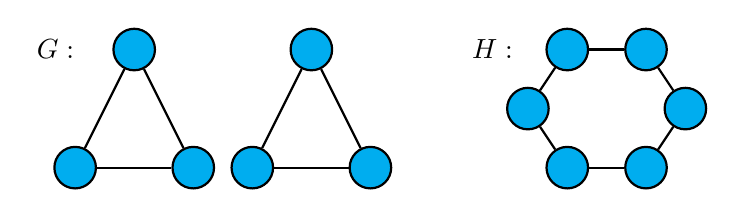
\begin{tikzpicture}

\tikzset{line/.style={draw,thick}}
\tikzset{arrow/.style={line,->,>=stealth}}
\tikzset{node/.style={circle,inner sep=0pt,minimum width=15pt}}

\draw (-1.0,0.75) node {$G:$};
\node[line,node,fill=cyan] (x1) at (0, 0.75) {};
\node[line,node,fill=cyan] (x2) at (-0.75, -0.75) {};
\node[line,node,fill=cyan] (x3) at (0.75, -0.75) {};

\path[line] (x1) to (x2);
\path[line] (x1) to (x3);
\path[line] (x2) to (x3);

\node[line,node,fill=cyan] (x1) at (2.25, 0.75) {};
\node[line,node,fill=cyan] (x2) at (1.5, -0.75) {};
\node[line,node,fill=cyan] (x3) at (3.0, -0.75) {};

\path[line] (x1) to (x2);
\path[line] (x1) to (x3);
\path[line] (x2) to (x3);

\draw (3.7 + 0.85, 0.75) node {$H:$};
\node[line,node,fill=cyan] (x1) at (3.75 + 1.25, 0) {};
\node[line,node,fill=cyan] (x2) at (4.25 + 1.25, 0.75) {};
\node[line,node,fill=cyan] (x3) at (5.25 + 1.25, 0.75) {};
\node[line,node,fill=cyan] (x4) at (5.75 + 1.25, 0) {};
\node[line,node,fill=cyan] (x5) at (5.25 + 1.25, -0.75) {};
\node[line,node,fill=cyan] (x6) at (4.25 + 1.25, -0.75) {};

\path[line] (x1) to (x2);
\path[line] (x2) to (x3);
\path[line] (x3) to (x4);
\path[line] (x4) to (x5);
\path[line] (x5) to (x6);
\path[line] (x6) to (x1);

\end{tikzpicture}